%! Author = erick-hdz
%! Date = 18/03/21

% Preamble
\documentclass{beamer}
\usetheme{Boadilla}

\title{My presentation}
\subtitle{Using beamer}
\author{Erick Hdz}
\institute{Sicuentame}
\date{\today}
% Packages
\usepackage{amsmath}
\usepackage{graphicx}

% Document
\begin{document}
    \begin{frame}
        \titlepage
    \end{frame}

    \begin{frame}
        \frametitle{Tabla de contenidos}
        \tableofcontents
    \end{frame}
    
    \section{¿Qué es la ciencia de datos?}
    \subsection{ sub a}

    \begin{frame}
        \frametitle{Title 1}
        some consideration
        \begin{itemize}
            \item<1-> Text visible on slide 1
            \item<2-> Text visible on slide 2
            \item<3-> Text visible on slide 3
            \item<4->Text visible on slide 4
        \end{itemize}
    \end{frame}

    \begin{frame}
        \frametitle{Data Science Schema}
        \begin{figure}
            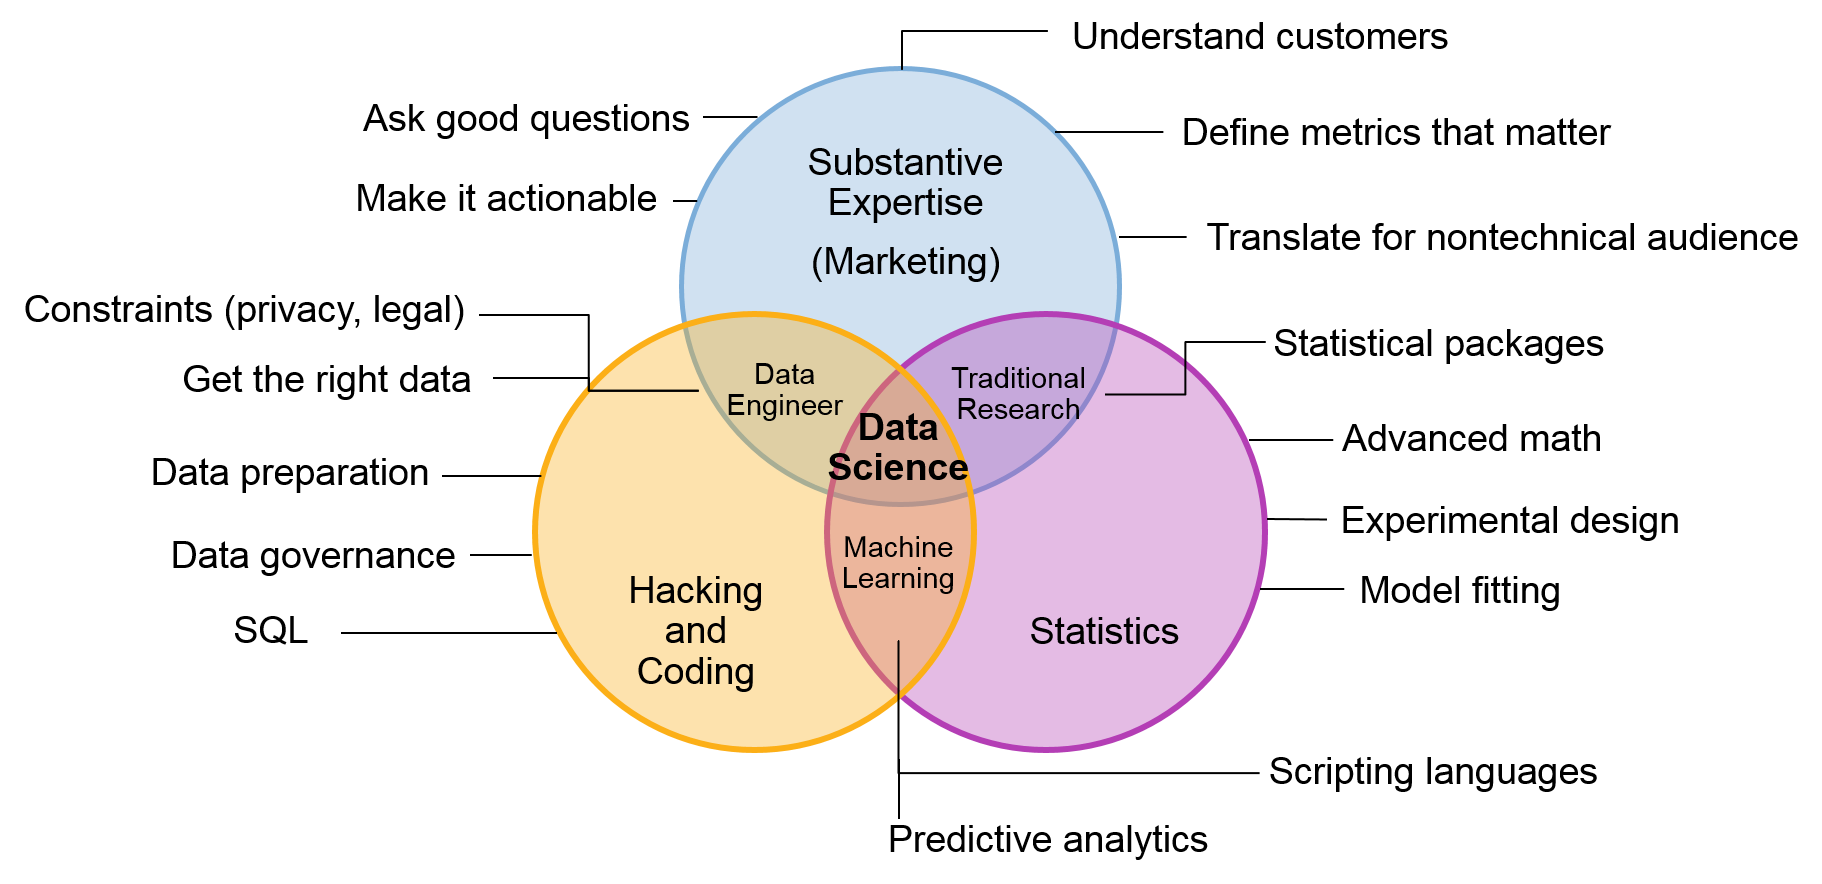
\includegraphics[scale=0.25]{datascience_skills_venn_diagram2}
            \caption{data science!}
        \end{figure}
    \end{frame}

    \subsection{ sub b}

    \begin{frame}
        \frametitle{Title 3}
        \begin{columns}
            \column{0.25\textwidth}
            Descripcion de lo que es ciencia de datos.
            \column{0.25\textwidth}
            Otra descripcion de ciencia de datos
            con implementacion en python con librerias de ciencia de datos.
            \column{0.25\textwidth}
            Algunas librerias escritas en python para la implementacion de ciencia de datos
        \end{columns}
    \end{frame}

    \section{Section 2}

    \begin{frame}
        \frametitle{Chatbots}
        Un chatbot es un servicio, con reglas regidas con máquinaria de inteligencia artificial,
        que hace una interacción con el cliente vía un chat.
    \end{frame}

    \section{Section 3}
     \begin{frame}
         \frametitle{Title 5}
         Some section of the content.
     \end{frame}


\end{document}